\documentclass[16pt]{beamer}
\usepackage[T1]{fontenc}
\usepackage[utf8]{inputenc}
\usepackage{graphicx}
\usetheme{Madrid}
\usecolortheme{beaver}
\usepackage{ragged2e}
\usepackage{etoolbox}

\apptocmd{\frame}{}{\justifying}{}
 
%Information to be included in the title page:
\title{Wstęp do uczenia maszynowego}
\subtitle{AdaLine i maszyna liniowa}
\author{Tomasz Derek}
\institute{KMS}
\date{Listopad 20, 2019}
 
\begin{document}
 
\frame{\titlepage}
 
\begin{frame}
\frametitle{Krótkie przypomnienie}
\begin{center}
\justifying
Na ostatnich zajęciach omawialiśmy perceptron. Powiedzieliśmy sobie również o funkcji aktywacji, a także o problemie minimalizacji funkcji błędu. Model perceptronu uczyliśmy za pomocą jednego z trzech algorytmów: simple learning algorithm, pocket learning algorithm, pocket learning algorithm with ratchet.
\end{center}
\end{frame} 
 
\begin{frame}
\frametitle{Ogólny zapis perceptronu progowego}
\[
    O(x_1, ..., x_n) = f(\sum_{i=1}^{n}x_iw_i + w_0)
\]
\begin{center}
    lub też
\end{center}
\[
    O(x_1, ..., x_n) = f(\sum_{i=1}^{n}x_iw_i - \theta)
\]
\end{frame} 
 
\begin{frame}
\frametitle{Funkcja progowa}
\[ f(x) =
  \begin{cases}
    -1       & \quad x < 0\\
    +1  & \quad x \geq 0
  \end{cases}
\]
\end{frame}

\begin{frame}
\frametitle{AdaLine}
\begin{center}
AdaLine - Adaptive Linear Neuron
\end{center}
\end{frame}

\begin{frame}
\frametitle{Główne różnice między Perceptronem a AdaLine}
\begin{itemize}
	\item Funkcja aktywacji
	\item Algorytm uczenia
\end{itemize}
\end{frame}

\begin{frame}
\frametitle{Zapis AdaLine}
\[
    O(x_1, ..., x_n) = \sum_{i=1}^{n}x_iw_i + w_0
\]
\begin{center}
    lub też
\end{center}
\[
    O(x_1, ..., x_n) = \sum_{i=1}^{n}x_iw_i - \theta
\]
\end{frame} 

\begin{frame}
\frametitle{Błąd}
\begin{center}
\[
\varepsilon = d - s
\]
\end{center}
gdzie \textbf{d} oznacza nasz oczekiwany sygnał wyjściowy, a \textbf{s} oznacza wyjście naszej sieci
\end{frame}

\begin{frame}
\frametitle{Dobór wag i problem minimalizacji błędu}
\[
E(w) = \frac{1}{2}\varepsilon^2 = \frac{1}{2}\left[d - s\right]^2 = \frac{1}{2}\left[d - (\sum_{i=1}^{n}x_iw_i - \theta)\right]^2
\]
\end{frame}

\begin{frame}
\frametitle{Dobór wag i problem minimalizacji błędu}
\begin{center}
WOW I CO TERAZ?
\end{center}
\begin{figure}[ht]

\includegraphics[scale=0.65]{./cry.jpg}
\end{figure}
\end{frame}

\begin{frame}
\frametitle{Algorytm spadku gradientowego}
\begin{itemize}
	\item Dana jest funkcja $f:R^n \to R$, która jest różniczkowalna
	\item Chcemy znaleźć jej minimum lokalne w sposób numeryczny
\end{itemize}
\end{frame}

\begin{frame}
\frametitle{Pochodna cząstkowa}
Pochodną cząstkową danej funkcji $f:R^n \to R$ po $x_i$ określamy jako:
\[
\frac{\partial f}{\partial x_i} \left(x_1, ..., x_n\right) = \lim\limits_{h \to 0} \frac{f(x_1, ..., x_{i-1}, x_i + h, x_{i+1}, ..., x_n) - f(x_1, ..., x_n)}{h}
\]
\end{frame}

\begin{frame}
\frametitle{Dobór wag i problem minimalizacji błędu}
\begin{figure}[ht]
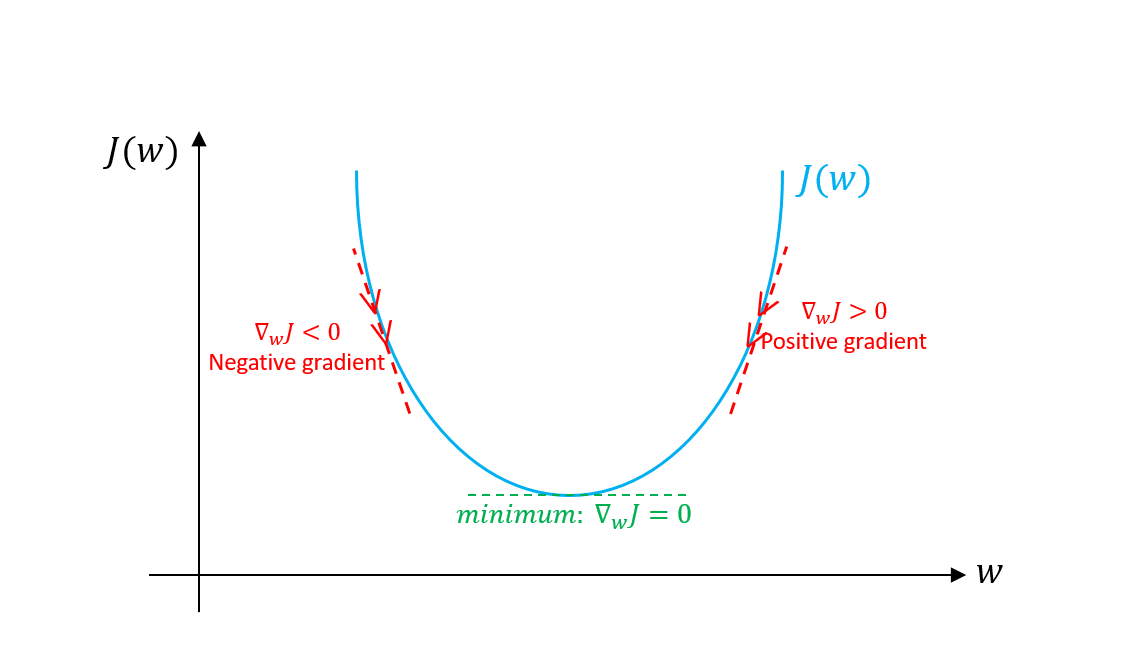
\includegraphics[scale=0.25]{./gradient.png}
\end{figure}
\end{frame}

\begin{frame}
\frametitle{Co to jest gradient?}
Gradientem pewnej funkcji sklarnej $f(x_1, ..., x_n)$ w układzie współrzędnych kartezjańskich nazywamy wektor, którego składowymi są pochodne cząstkowe funkcji $f$.
\[
	\nabla f = \left[\frac{\partial f}{\partial x_1}, ..., \frac{\partial f}{\partial x_n} \right]
\]
Innymi słowy gradient wskazuje w którą stronę i funkcja $f$ rośnie w wybranym przez nas punkcie.
\end{frame}


\begin{frame}
\frametitle{Algorytm spadku gradientowego}
Z angielskiego \textit{Gradient Descent Algorithm} w skrótcie GDA
\begin{itemize}
	\item Chcemy znaleźć minimum funkcji f
	\item Obliczamy gradient pochodnych cząstkowych
	\item Robimy krok w przeciwnym kierunku
\end{itemize}
\end{frame}

\begin{frame}
\frametitle{Algorytm uczenia AdaLine}
Ze względu na fakt, że nasza funkcja jest różniczkowalna, zastosujemy do niej metodę największego spadku gradientu:
\[
	w_i = w_i - \eta \frac{\partial E(w_i)}{\partial w_i} = w_i + \eta(d-s)x_i
\]
Możemy to zapisać w powyższy sposób ze względu na fakt, iż:
\[
	\frac{\partial E(w_i)}{\partial w_i} = \frac{\partial E(w_i)}{\partial s} * \frac{\partial s}{\partial w_i}
\]
Ponieważ $s$ jest funkcją liniową względem wektora wag, więc możemy zapisać:
\[
	\frac{\partial s}{\partial w_i} = x_i
\]
\end{frame}

\begin{frame}
\frametitle{Algorytm uczenia AdaLine c.d.}
Ponadto:
\[
	\frac{\partial E(w_i)}{\partial s} = -(d-s)
\]
$\delta = (d-s)$
Wtedy wzór przyjmuje postać:
\[
w_i = w_i + \eta \delta x_i
\]
\end{frame}

\begin{frame}
\frametitle{Model neuronu sigmoidalnego}
Model neuronu sigmoidalnego nie różni się dużo od modeli AdaLine czy też Perceptronu. Różnica polega na zastosowaniu innej funkcji aktywacji, a dokładniej funkcji sigmoidalnej. Model ten uczymy na zasadzie algorytmu największego spadku gradientu:
\[
	w_i = w_i - \eta \frac{\partial E(w_i)}{\partial w_i} = w_i + \eta(d-f(s))f'(s)x_i
\]
\end{frame}

\begin{frame}
\frametitle{Algorytm}
\begin{itemize}
	\item Losujemy wagi
	\item Losujemy przykład
	\item Obliczamy pobudzenie wagi
	\item Korygujemy wagi
	\item Kończymy przechodząc przez odpowiednią ilość iteracji. W przeciwnym wypadku wracamy do 2.
\end{itemize}
\end{frame}

\end{document}https://github.com/HyperScypion/KMS_Neural_Networks/tree/master/challenges/fourth_lecture/presentation